\documentclass{ieeeaccess}
\usepackage{bbm}
\usepackage{cite}
\usepackage{amsmath,amssymb,amsfonts}
\usepackage{graphicx}
\usepackage{textcomp}
\usepackage{hyperref}
\usepackage[noend]{algpseudocode}
\usepackage{algorithm}
\usepackage{subfig}
\usepackage{booktabs}
\usepackage{adjustbox, soul, color}
\usepackage{array}
\usepackage{float}
\def\BibTeX{{\rm B\kern-.05em{\sc i\kern-.025em b}\kern-.08em
    T\kern-.1667em\lower.7ex\hbox{E}\kern-.125emX}}
\begin{document}
\history{Date of current version October 11, 2024.}
\doi{00.0000/ACCESS.2024.DOI}
\title{Enhancing Fractographic Failure and Fatigue Analysis of Titanium Alloys in Additive Manufacturing Using Image Processing and Deep Learning}


\author{\uppercase{Or Haim Anidjar\authorrefmark{1,2,3,4}, Mor Mega\authorrefmark{5}, \uppercase{Yonatan Boritski \authorrefmark{1} and Avichay Mazin\authorrefmark{1}.}}
\address[1]{School of Computer Science, Ariel University, Israel.}
\address[2]{Kinematics and Computational Geometry Lab (K\&CG), Ariel University, Israel.}
\address[3]{Ariel Cyber Innovation Center (ACIC), Ariel University, Israel.}
\address[4]{Data Science and Artificial Intelligence Research Center, Ariel University, Israel.}
\address[5]{School of Mechanical Engineering and Mechatronics, Ariel University, Golan Heights 1, 4077625, Ariel, Israel.}}

%\tfootnote{This paragraph of the first footnote will contain support 
%information, including sponsor and financial support acknowledgment. For 
%example, ``This work was supported in part by the U.S. Department of 
%Commerce under Grant BS123456.''}


\begin{abstract}
Additive Manufacturing (AM) has revolutionized the production of complex components, offering unparalleled design flexibility and cost efficiency. However, the fatigue characteristics of AM-produced titanium alloys remain underexplored. This study proposes an innovative approach to automate the analysis of fatigue fracture surfaces in Ti-6Al-4V specimens using image processing and computer vision techniques. The method leverages the U-Net architecture for image segmentation and heatmap analysis to identify fatigue crack propagation areas. The proposed approach is designed to enhance the understanding of material failure mechanisms, predict stress intensity factors, and flow stresses, and facilitate quality control in AM processes. The dataset comprises 63 Scanning Electron Microscope (SEM) images of Ti-6Al-4V fatigue specimens, categorized by print quality. The dataset includes duplicated images from the upper and lower surfaces of specimens, providing a comprehensive examination of fracture patterns. The dataset is meticulously structured to support machine learning analysis, enabling the identification and analysis of fracture patterns and material defects. The proposed approach is expected to enhance the reliability of failure analysis, provide valuable insights into material failure mechanisms, and guide improvements in material design and manufacturing processes. The study's findings are anticipated to contribute significantly to the field of materials science, particularly in understanding the fatigue behavior of aerospace materials. The dataset and framework of the algorithms used in this study are publicly available, facilitating further research and development in the field of materials science.
\end{abstract}

\begin{keywords}
Fractography, Computer Vision, Image Processing, Fatigue Failure, Additive Manufacturing, Deep Learning.
\end{keywords}

\titlepgskip=-15pt

\maketitle



\section{Introduction}
\label{introduction}
Additive Manufacturing (AM) is a process that enables the fabrication of parts layer by layer using 3D models. This technology, a cornerstone of the third industrial revolution, offers unlimited opportunities for intricately designed products and significantly reduces production costs. One of the main advantages of AM is the elimination of the need for molds, which significantly reduces production costs ~\cite{herzog2016additive}.

Titanium alloys are highly advanced structural materials known for their exceptional properties, such as resistance to corrosion, strength-to-weight ratios, fracture toughness, high fatigue resistance, and compatibility with composites ~\cite{qian2016additive}. However, their dynamic performance and fatigue characteristics remain comparatively scanty ~\cite{debroy2018additive,gorsse2017additive}.

\subsection{Fatigue Characteristics of Additive Manufactured Alloys}
Traditional subtractive manufacturing (SM) for manufacturing Ti-6Al-4V alloys is inefficient and resource-intensive, leading to increased costs and waste ~\cite{peng2017toward}. Advanced techniques like Selective Laser Melting (SLM) and Electron Beam Melting (EBM) reduce waste and time by producing near-net-shape components from CAD models, especially for complex geometries and lightweight aircraft components ~\cite{fatimah2013sustainable}. EBM, another AM technique, operates on a much wider scale compared to SLM.

The Selective Laser Melting (SLM) process has intrinsic limitations, such as the formation of uncontrolled defects like porosity, cracks, and inclusions, which can significantly affect the mechanical properties of the final product. In fracture mechanics, there has been a shift from focusing on static properties, like strength and toughness, to analyzing dynamic properties, such as fatigue and fracture behavior. This shift is important for understanding how materials perform under dynamic loading conditions like heat, pressure, vibration, and cyclic loading.


Fatigue failure of engineering components and structures results from progressive fracture caused by cyclic or fluctuating loads. Fatigue is an important potential cause of mechanical failure because most engineering components or structures can be subjected to cyclic loads during their lifetime.
Characteristic fatigue fracture features that can be visually discerned under low magnification are then described.
Typical microscopic features observed on structural metals are presented.

The flow stress and stress intensity factor are critical parameters for predicting the final failure of a specimen under cyclic fatigue loading. The flow stress parameter, \(\sigma_{\text{net}}\), is related to the applied force and the uncracked area of the specimen. When \(\sigma_{\text{net}}\) reaches the failure stress, \(\sigma_f\), the specimen fails, and crack initiation occurs. The stress intensity factor, \(K_I\), is linked to the fracture toughness, \(K_{IC}\), of the material. When \(K_I\) reaches \(K_{IC}\), crack propagation occurs. Once the crack reaches the critical size, the specimen fractures completely. Understanding \(\sigma_{\text{net}}\) and \(K_I\) is crucial for predicting material failure, designing safe structures, and selecting appropriate materials. These parameters illustrate internal resistance and stress concentration around cracks, thereby preventing catastrophic failures and enhancing material robustness.

An abbreviated summary of fatigue processes and mechanisms: fatigue crack initiation, propagation, and final fracture.
In Stage I, the initiation stage, cracks propagate along high shear stress planes (45 degrees) with microstructural barriers like grain boundaries decelerating the process. Surface treatments such as shot peening and surface rolling increase the number of microstructural barriers, helping to prevent fatigue cracks. Stage II begins with an increase in the stress intensity factor, \(K\), which predicts the stress state near the crack tip due to remote load or residual stresses. The value of \(K\) depends on sample geometry, crack size and location, and load distribution. As \(K\) increases from crack growth or higher applied loads, slips develop near the crack tip. Stage III is the unstable part of crack growth, occurring when \(K_{\text{max}}\) approaches \(K_{IC}\). This leads to rapid material failure due to cyclic static mode failures, with significant sensitivity to microstructure, load ratio, and stress state. The instability of Stage III limits the information extractable from its surface \cite{newman1981empirical}.

\subsection{Computer Vision and Machine Learning in Additive Manufacturing}
Computer vision and machine learning techniques have been increasingly employed in the field of additive manufacturing to address challenges related to material characterization, defect detection, and failure analysis. During the additive manufacturing (AM) process, materials may experience changes in their properties, potentially leading to failures and defects. To address these challenges, researchers typically investigate the process in three chronological stages:
\begin{itemize}
    \item \textbf{Preprocessing.} Gathering and analyzing material characteristics before the AM process begins. In ~\cite{miyazaki2019image}, the authors conducted a study on the influence of heat treatment during the SLM process on the micro-structure and mechanical properties of Ti-6Al-4V. They utilized machine learning techniques for image segmentation and analysis.
    \item \textbf{In-Process Monitoring.} Monitoring in additive manufacturing involves using various sensors to collect real-time data on production tasks, including indicators, signals, and images, to detect defects and ensure process control. Laser welding is an additive manufacturing process commonly used for materials welding, especially in the automated welding of small components, within sectors such as medical devices, aerospace components, and electronics. In~\cite{cai2023real}, an CNN model was developed, along with an adaptive fusion image method to eliminate some of the noise in the images, to monitor the penetration state during laser keyhole welding, ensuring the quality of the welding process.
    \item \textbf{Postprocessing.} Evaluating and analyzing the material after the AM process is completed. Applying ML techniques to achieve accurate classification and segmentation of defects, similar to the method used by Dung et al. who constructed a deep FCN with VGG16 as the backbone to achieve crack detection by means of semantic segmentation of concrete images \cite{pu2022autonomous}.
\end{itemize}

\subsection{Our Contribution}
This study focuses on the post-processing stage, analyzing the stress intensity factor and flow stress of the Ti-6Al-4V alloy after the additive manufacturing (AM) process. An innovative approach is proposed to automate the analysis of fatigue fracture surfaces in these specimens, based on the U-Net architecture and heatmap analysis, can be further refined and extended to address a wide range of material science challenges, including:

\begin{itemize}
    \item \textbf{Material Characterization.} The automated processes can be applied to a variety of materials, especially metals, to characterize their microstructures and fatigue failure modes under cyclic loads, and to calculate stress intensity factors, flow stresses, and other critical parameters.
    \item \textbf{Quality Control.} The automated analysis can be integrated into industrial quality control processes to detect defects, cracks, and other anomalies in manufactured components, ensuring product reliability and safety.
    \item \textbf{Failure Analysis.} The detailed fracture analysis enabled by the U-Net model and heatmap techniques can provide valuable insights into the root causes of material failures, guiding improvements in material design and manufacturing processes.
    \item \textbf{Research and Development.} The automated segmentation and analysis methods can accelerate research and development efforts by providing rapid and accurate feedback on material properties and performance, facilitating the design of new materials with enhanced characteristics.
\end{itemize}


\section{Related Work}
 The integration of computer vision in the field of fracture mechanics, particularly in the analysis of metal fractures, has evolved significantly over recent years.
In its early stages, the approach primarily relied on Scanning Electron Microscope (SEM) images and conducting manual classification efforts.
However, the traditional process is manual, labor-intensive, and prone to human error.
Automating this process and developing quantitative methods for studying fracture surfaces is a major challenge but has significant industrial and scientific potential.
Automated fractography could enhance the reliability of failure analysis and uncover new insights into material failure mechanisms.

Early applications in fracture mechanics prioritized image processing over the more advanced computer vision and machine learning techniques.
These initial approaches were designed to enhance features in images of fracture surfaces captured by SEM and optical microscopy, with a greater emphasis on qualitative rather than quantitative analysis.
Fundamental techniques employed in these efforts included spatial domain methods like texture analysis and the Gray Level Co-occurrence Matrix (GLCM) for fractal analysis.
In \cite{zain2009enhancement}, the authors experimented with various spatial filtering techniques such as mean, median, Gaussian, and Wiener filters to enhance the quality of the identification of the fracture image.
In the engineering field, another set of experiments can be observed In \cite{das2011characterization}, where the changes on the surface are effectively characterized using these methods.
Furthermore, some of these techniques also incorporated transform domain methods, such as Fourier transform, wavelet transform, and Gabor transform.
In another study, In \cite{hu2017automation}, the authors employed edge detection and peak-finding algorithms to determine the progression marks associated with fatigue crack growth.

These methods were applied to optical and Scanning Electron Microscopy (SEM) images to classify and characterize fracture surfaces.
However, these methods often required additional user input and assumptions, which limited their robustness and applicability, especially for complex surfaces.

Recent developments have seen the use of machine learning and artificial intelligence in materials characterization, including micro-structure classification and defect analysis.
Promising machine learning methods like artificial neural networks and support vector machines have played a pivotal role in classifying observed fractures, yielding promising results in materials characterization.
Some notable achievements in this area include the use of a complex CNN architecture known as Unet,
as demonstrated In \cite{tsopanidis2020toward}, where an accuracy of 71.2 percent in Intersection over Union (IOU) was achieved for triple-class classification,
distinguishing inter-granular and trans-granular fracture events from scanning electron microscope images.
Another article compared a more intricate Unet neural network architecture, reaching an accuracy of 86 percent in the Dice score accuracy metric for the segmentation task of detecting dimple fractures \cite{sinha2021deep}.

A prominent trend has emerged in recent times where a fusion of traditional image processing methods and cutting-edge AI techniques has been observed.
In these approaches, a pivotal role is played by feature extraction during the prepossessing phase, enhancing the salient characteristics within images.
As exemplified In \cite{naik2019identification}, researchers combined texture recognition algorithms, specifically the Local Binary Pattern (LBP), with the classical machine algorithm called Linear Discriminant Analysis (LDA). This innovative combination allowed them to identify the fracture type and its area in both brittle and ductile materials by leveraging the uniqueness of texture features, achieving an impressive accuracy rate of 94 percent.
Another notable example is presented In \cite{bastidas2016fractographic}, where SVM classification was employed to classify three different types of fractures in crystalline materials.
In the field of fracture mechanics, certain techniques leverage the connection between computer vision and machine learning for fracture surface analysis. Feature extraction methods, such as edge detection using the Sobel operator, can enhance image quality and denoise the image, isolating the necessary features and improving the accuracy of models. For instance, Wang et al. (2019) introduced an improved Sobel operator combined with Otsu thresholding for feature extraction in the classification of cracks in concrete bridge structures \cite{wang2019research}. This method utilized image vertical and horizontal projection profiles to classify four types of cracks.
Inspired by this enhancement method, a comparative analysis was conducted to assess the performance of these contrast enhancement methods along with a Deep Convolution Neural Network (DCNN) for a binary classification task. This approach achieved a 16.8\% improvement in accuracy over images without enhancement, as demonstrated by Bhalaji et al. (2024) \cite{bhalaji2024transfer}.

An advancement in this research lies in the integration of the localization problem with the feature extraction phase.
As demonstrated In \cite{zhang2023automated}, a remarkable achievement was reached with a detection rate of up to 92 percent in terms of the F1 score for detecting bridge cracks.
This approach was developed by segmenting the process into three distinct phases: initially selecting specific regions, then extracting features using methods like SIFT and HOG, and finally applying the YOLO neural network architecture for precise object localization and detection.

Our proposed method is designed to automate the extensive labor involved in analyzing the properties of fatigue fracture surfaces in Ti-6Al-4V specimens produced through additive manufacturing. The approach utilizes a multi-stage process, including image preprocessing, feature extraction, classification and crack front detection and stress analysis.
\begin{itemize}
    \item \textbf{Image Preprocessing.} This stage involves removing extraneous metadata and resizing images to a uniform resolution, ensuring that the learning algorithms focus on the relevant features of the specimens.
    
    \item \textbf{Feature Extraction.} The magnitude of image gradients is calculated, producing heatmaps using a Sobel transform. These heatmaps enhance the images for easier analysis and enable the identification of fatigue crack propagation areas.
    
    \item \textbf{Classification.} A specialized neural network architecture, UNet, is used for image segmentation. This network classifies and identifies the contours of fatigue crack propagation areas based on the heatmap images and the overall specimen contour in the original image.
    
    \item \textbf{Crack Front Detection and Stress Analysis.} Computer vision techniques are employed to detect the elliptical crack front, enabling the calculation of both the stress intensity factor and the flow stress of the specimen based on the detected contours.
\end{itemize}
In addition, the dataset and the framework of the algorithms used in this study are present.

\section{Terms and Definitions}

\subsection{Mechanical basic terms}  \label{sec:Basic terms}

 
Two failure criteria may be used to predict the final failure of a specimen subjected to cyclic fatigue loading. The first criterion is related to the flow stress parameter \(\sigma_{net}\), and the second is related to the stress intensity factor \(K_{I}\). Once one of these parameters reaches a critical value, failure is expected. The model used here to determine the flow stress in a bar specimen tested in cyclic fatigue is presented in Section~\ref{Subsec: Flow stress calculation model}.
In Section~\ref{Subsec: Stress intensity factors calculation model}, several closed-form solutions for the determination of \(K_I\) are introduced and the best one is chosen \cite{shin2004experimental}.   


\subsubsection{Fractographic image analysis description}
\label{Subsec: Fractographic image analysis}

\subsubsection{Flow stress calculation model}
\label{Subsec: Flow stress calculation model}
\begin{figure*}[!t]
  \begin{center}
  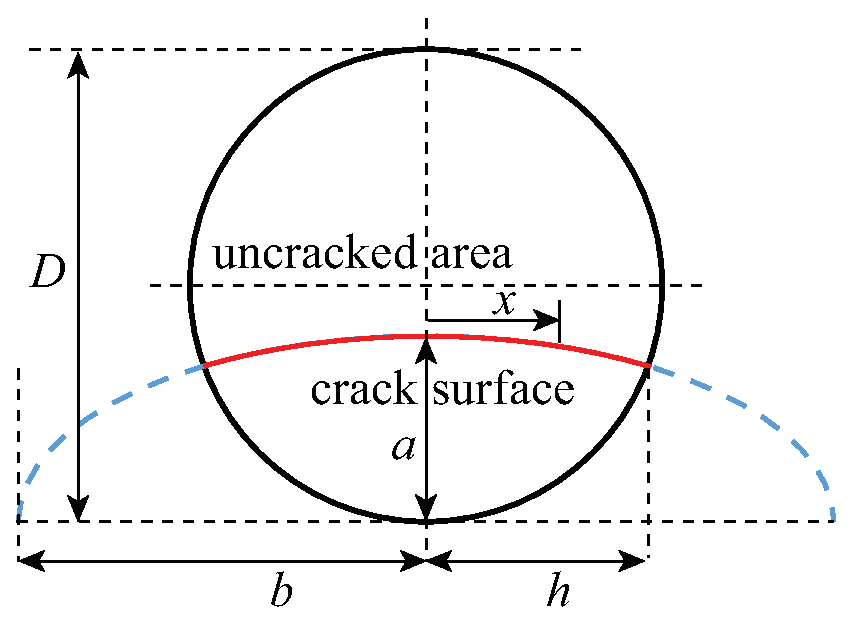
\includegraphics[width=0.5\textwidth]{elliptical_surface_crack.eps}
  \caption{Schematic view of an elliptical crack.}
  \label{fig:elliptical_crack}
   \end{center}
\end{figure*}

One known failure criterion is based on the calculated flow stress $\sigma_{net}$. Once this parameter reaches the failure stress $\sigma_{f}$, the final failure will occur.

The failure stress \(\sigma_{f}\) is related to the ligament area, defined as the uncracked area illustrated in Fig.~\ref{fig:elliptical_crack}. For a specific material, the value of \(\sigma_{f}\) is given by \cite{kanchanomai2004low}
%
\begin{equation}
    \sigma_{f} = \frac{\sigma_Y + \sigma_{UTS}}{2}
\end{equation}
%
where \(\sigma_Y\) is the yield stress and \(\sigma_{UTS}\) is the ultimate stress of the material. 

The flow stress, \(\sigma_{net}\), is a function of the applied force and the uncracked area, namely,
%
\begin{equation}
\label{eq:sig_net}
\sigma_{net}= \displaystyle\frac{\sigma_{max} A_0}{A_{\textit{uncracked area}}}
\end{equation}
%
where $\sigma_{max}$ is the maximum applied stress in each fatigue cycle, \(A_0\) is the total area of the specimen surface, and \(A_{\text{uncracked area}}\) is the ligament area illustrated in Fig.~\ref{fig:elliptical_crack}. Once \(\sigma_{net}\) reaches the value of \(\sigma_f\), the specimen will fail.
%
%

\subsubsection{Stress intensity factor calculation model}
\label{Subsec: Stress intensity factor calculation model}
%
%
\begin{table}[t!]
\caption{Tabulated values of $M_{i,j,k}$ in eq.~(\ref{eq:F_I}). \strut}
\label{tab:M_ijk}      % Give a unique label
\resizebox{\columnwidth}{!}{
\begin{tabular}{cccclccclccc}
\noalign{\bigskip}\hline\noalign{\smallskip}
  &          & k=0       &           &  &          & k=1       &          &  &         & k=2      &           \\ \noalign{\bigskip}\hline\noalign{\smallskip}
j & i=0      & 1         & 2         &  & i=0      & 1         & 2        &  & i=0     & 1        & 2         \\
0 & 1.095    & -1.177    & 0.725     &  & 0.113    & 0.271     & -0.388   &  & -0.896  & 0.904    & 0.008     \\
1 & -1.336   & 17.924    & -17.427   &  & 1.824    & -11.649   & 10.074   &  & 3.092   & 0.701    & -4.883    \\
2 & 13.108   & -137.252  & 134.652   &  & -21.709  & 98.358    & -80.088  &  & -4.197  & -32.641  & 55.092    \\
3 & -43.689  & 545.816   & -551.902  &  & 105.483  & -415.027  & 328.165  &  & -13.255 & 204.104  & -305.079  \\
4 & 134.868  & -1223.334 & 1239.493  &  & -271.225 & 982.713   & -772.921 &  & 51.548  & -568.407 & 916.962   \\
5 & -242.653 & 1541.587  & -1548.537 &  & 387.47   & -1329.634 & 1055.952 &  & -59.329 & 857.543  & -1545.428 \\
6 & 254.093  & -1006.656 & 969.388   &  & -290.024 & 961.893   & -784.581 &  & 13.481  & -657.659 & 1372.595  \\
7 & -108.196 & 264.206   & -227.132  &  & 88.387   & -288.565  & 245.798  &  & 10.854  & 191.57   & -485.556  \\ 
\hline\noalign
\end{tabular}
}
\end{table}
An additional known failure criterion is based on the stress intensity factor $K_I$ value. Once this parameter reaches the fracture toughness $K_{Ic}$ of the tested material, the crack will propagate, and final failure will occur. The critical stress intensity factor or fracture toughness value \(K_{Ic}\) is reached once the crack approaches a critical size. 



In~\cite{toribio2009automated}, it was demonstrated that the crack front in a fatigue bar specimen may be treated as an ellipse with the center located at the specimen surface, as illustrated in Fig.~\ref{fig:elliptical_crack}. The parameters $a$ and $b$ are the major and minor diameters of the ellipse in Fig.~\ref{fig:elliptical_crack}, respectively. These dimensions represent the depth and width of the crack, respectively. The parameter $D$ is the total specimen diameter, $x$ is a chosen coordinate between 0 and $h$ where $h$ is the horizontal distance between the center of the ellipse and the intersection between the ellipse and the specimen outer surface. It may be noted that the axis of symmetry of the ellipse is the same as the axis of symmetry of the bar and the center of the ellipse is on the edge of the rod. All parameters are shown in Fig.~\ref{fig:elliptical_crack} and may be used to calculate $K_I$.

Next, several closed-form solutions are presented and the best one is chosen. In~\cite{valiente1980criterios}, the first closed-form solution was introduced. This form was only for a straight front crack ($b$ limit to infinity). The value of $K_I$ is calculated only at the center of the crack front. 
In~\cite{astiz1986incompatible}, a closed-form solution is introduced for an elliptical crack front; but $K_I$ is found only in the center of the crack front. In~\cite{couroneau1998simplified,carpinteri1992elliptical} two closed-form solutions were presented, one at the crack front center, shown as point A in Fig.~\ref{fig:elliptical_crack}, and another for the end of the crack front, shown as point G in Fig.~\ref{fig:elliptical_crack}. In \cite{shin2004experimental} a closed-form solution was found based on the FE method and the virtual crack extension technique~\cite{hellen1975method}. The solution was found as a function of $a$, $b$, and $x/h$ the location along the crack front, as shown in Fig.~\ref{fig:elliptical_crack}.
Another solution that uses these three parameters~\cite{shih2002stress} was found to produce negative results. A detailed review of these solutions and other solutions may be found in~\cite{toribio2009automated}.
It was found~\cite{toribio2009automated} that the best closed-form solution for the problem in this research is~\cite{shih2002stress}.


In~\cite{shin2004experimental}, the closed-form solution is based on the FE method and the virtual crack extension technique~\cite{hellen1975method}.  The calculation of \(K_I\) is proposed as
%
\begin{equation}
\label{eq:K_I__F_I}
K_{I}=F_I \sigma_0 \sqrt{\pi a}
\end{equation}
%
where $F_I$ is a function of $a, b, D, h$ and $x$ given as
%
\begin{equation}
\label{eq:F_I}
F_{I}=\sum^{2}_{i=0} \sum^{7}_{j=0}\sum^{2}_{k=0} M_{ijk}\left(\frac{a}{b}\right)^i  \left(\frac{a}{D}\right)^j  \left(\frac{x}{h}\right)^k\;\;.
\end{equation}
In eq.~(\ref{eq:F_I}) the coefficients $M_{ijk}$ were determined from FEAs in \cite{shin2004experimental} and presented in Table~\ref{tab:M_ijk}.



\subsection{Neural Network Terms}
\label{subsec:network_terms}
computational models inspired by the human brain's neural structure. They consist of interconnected units called neurons, organized into layers: the input layer (which receives the data), hidden layers (which process the data), and the output layer (which produces the final output). Each connection between neurons has an associated weight and bias, which are adjusted during training to minimize the error in the network's predictions \cite{lecun2015deep}.
The learning process of a neural network involves several key steps:
\begin{itemize}
    \item \textbf{Forward Pass.} Input data is passed through the network, layer by layer, to generate predictions. Each neuron performs a weighted sum of its inputs and passes the result through an activation function to introduce non-linearity.
    \item \textbf{Error Calculation.} The difference between the predicted output and the actual output (the error) is calculated using a loss function. Common loss functions include Mean Squared Error (MSE) for regression tasks and Cross-Entropy Loss for classification tasks \cite{goodfellow2016deep}.
    \item \textbf{Backward Pass (Backpropagation).} The error is propagated backward through the network. The gradients of the loss function with respect to each weight are computed using the chain rule of calculus. These gradients indicate how much each weight contributes to the overall error \cite{rumelhart1986learning}.
    \item \textbf{Weight Update.} The weights and biases are updated using an optimization algorithm, such as Stochastic Gradient Descent (SGD) or Adam, to reduce the error. This process iterates until the network's predictions are sufficiently accurate \cite{kingma2014adam}.
\end{itemize}
Optimization algorithms like Adam further enhance the training process by adapting the learning rate for each parameter, making the training more efficient and effective \cite{kingma2014adam}.
Neural networks have demonstrated remarkable performance in various tasks. For instance, in image recognition, neural networks can learn to identify and classify objects within images with high accuracy, as evidenced by the success of deep residual networks \cite{he2016deep}. Similarly, in natural language processing, neural networks have enabled significant advancements in understanding and generating human language, as showcased by the development of transformer models \cite{vaswani2017attention}. Furthermore, neural networks are pivotal in predictive analytics, where they uncover complex patterns and relationships within data, crucial for making accurate predictions \cite{schmidhuber2015deep}.
\subsection{Description of U-Net Architecture}
U-Net is a neural network architecture specifically designed for image segmentation tasks \cite{ronneberger2015u}. It is composed of two main parts: the contracting path and the expansive path, connected by skip connections.
\subsubsection{Contracting Path}
The contracting path functions like a standard convolutional neural network (CNN). It consists of repeated application of convolutional layers, each followed by a rectified linear unit (ReLU) activation function and a max pooling operation. The convolutional layers capture features such as edges and textures, while max pooling reduces the spatial dimensions of the image, preserving essential features. This path captures the context and down-samples the image to a lower resolution while increasing the number of feature channels.
\subsubsection{Expansive Path}
The expansive path rebuilds the image to its original resolution. It uses transposed convolutions (or upsampling) to increase the size of the feature maps. Each upsampling step is followed by a concatenation with the corresponding feature map from the contracting path via skip connections, ensuring that detailed information is preserved. The combined feature maps undergo additional convolutions to refine the segmentation \cite{ronneberger2015u}.
Skip connections play a crucial role by directly linking corresponding layers in the contracting and expansive paths. This direct connection helps retain fine-grained details that might otherwise be lost during downsampling, ensuring precise and detailed segmentations.
\begin{figure*} [!t]
    \centering 
    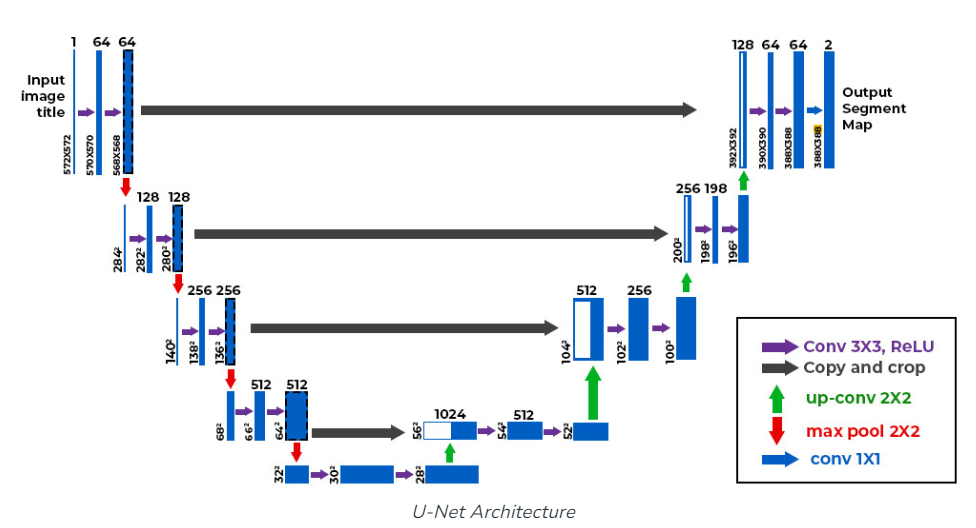
\includegraphics[width=0.9\textwidth]{figures/UNet.png}
\caption{Illustration of the U-Net architecture, showcasing the contracting path on the left side and the expansive path on the right side \cite{ronneberger2015u}.}
\label{fig:unet_architecture}
\end{figure*}
\subsection{Image Segmentation and Evaluation Metrics}
Image segmentation is the process of dividing an image into distinct regions, often for the purpose of identifying and classifying objects within the image. U-Net is particularly effective for segmentation tasks due to its ability to capture context and detail simultaneously.
Evaluating the performance of image segmentation models is crucial. Common metrics include:
\begin{itemize}
    \item \textbf{Dice Coefficient.} This metric measures the overlap between the predicted segmentation and the ground truth. As seen in prior research, it is calculated as:
    \[
    \text{Dice} = \frac{2|X \cap Y|}{|X| + |Y|}
    \]
    where \(X\) is the predicted segmentation and \(Y\) is the ground truth. A higher Dice coefficient indicates better segmentation performance \cite{milletari2016v}.
    \item \textbf{Intersection over Union (IoU).} Also known as the Jaccard index, this metric compares the overlap between the predicted segmentation and the ground truth relative to their combined area. It is formulated as:
    \[
    \text{IoU} = \frac{|X \cap Y|}{|X \cup Y|}
    \]
    where \(X\) and \(Y\) are the predicted segmentation and the ground truth, respectively. Higher IoU values indicate more accurate segmentation \cite{rahman2016optimizing}.
\end{itemize}
These metrics help quantify how well the model's segmentation matches the true segmentation, providing a clear measure of accuracy.

\section{Dataset} \label{Sec:dataset}

The dataset utilized in this research comprises 63 Scanning Electron Microscope (SEM) images of Ti-6Al-4V alloy fatigue specimens. Each image is captured at a resolution of 4576 by 4096 pixels, enabling detailed examination of the specimens over an area of 5.5 mm with a pixel size of approximately 1.34 $\mu$m, as such a fine resolution is crucial because it enables the observation of minute details and microstructural features, which are essential for understanding the material’s fatigue behavior at a microscopic level.
This is particularly important for subsequent analysis phases, including image preprocessing and computer vision feature extraction stages, where preserving all details without information loss is critical, and resolution manipulation is unnecessary.
The dataset is organized into three categories based on the print quality recommended by the manufacturer: 30 images in P1 for standard printing, 21 in P2 for enhanced quality, and 12 in P3 indicating lower quality. These groupings reflect different levels of manufacturing precision, which may be relevant for specific analyses.
This approach enriches the dataset with diverse specimens, enabling a comprehensive examination of fatigue fracture surfaces across various print qualities and facilitating a more nuanced understanding of the material's fatigue behavior under different conditions.
Detailed documentation on specimen production and experimental setups, as referenced in previous work \cite{navickaite2022efficient}, provides essential background for understanding the context of these SEM images.


\begin{figure}[ht!]
  \centering
  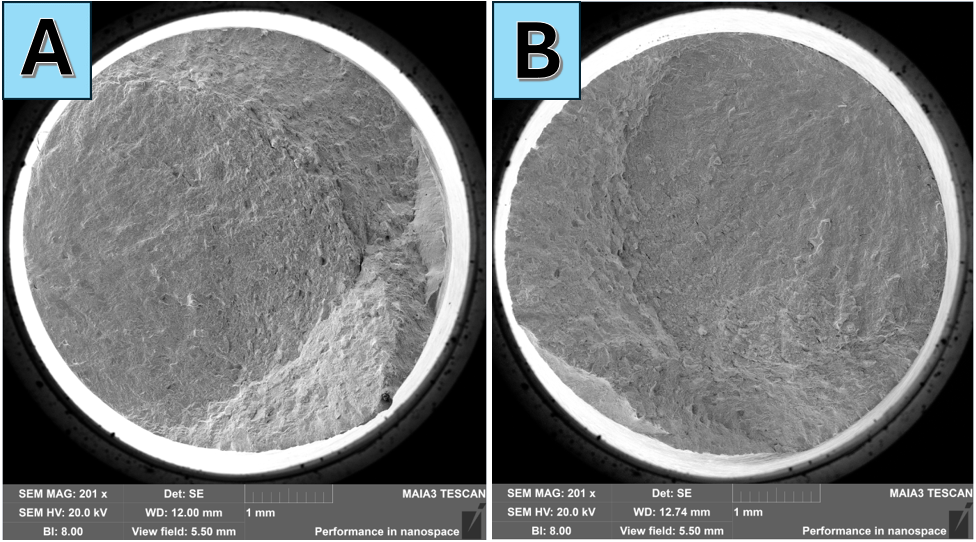
\includegraphics[width=0.5\textwidth]{figures/side_by_side.png}
  \caption{SEM images of a Ti-6Al-4V fatigue specimen from two opposing viewpoints (A and B), showcasing the fracture surfaces from the lower and upper surfaces at different angles.}
  \label{same_material_from_both_sides}
\end{figure}

\paragraph{Inclusion of Duplicated Images}
A significant feature of this dataset is the inclusion of duplicated images for certain specimens, which were captured from the upper and lower surfaces of the specimens at different angles. This duplication is instrumental in providing a more holistic examination of the material's structural integrity and failure mechanisms, enhancing the understanding of fatigue fracture surfaces, as well as enriching the dataset with a broader range of fracture patterns and features.  Figure~\ref{same_material_from_both_sides} illustrates this approach by displaying SEM images of a Ti-6Al-4V fatigue specimen from two contrasting viewpoints, labeled A and B, which showcase both the lower and upper surfaces at different angles, of an identical specimen.

\paragraph{Dataset Design for Machine Learning Analysis}
The dataset is meticulously structured to support machine learning endeavors, particularly for the identification and analysis of fracture patterns and material defects. The precise categorization and comprehensive documentation of the images are crucial for facilitating accurate algorithmic training and validation. These steps are fundamental in developing robust predictive models that can reliably forecast material failures.

This well-organized dataset serves not only the specific objectives of this research but also enhances the broader field of materials science. It offers valuable insights into the mechanical properties and failure mechanisms of aerospace materials, thereby contributing significant knowledge to the scientific community. Such contributions are vital for advancing understanding and technology in material durability and safety.


\section{Our Approach} \label{Our Approach}
\subsection{Preliminary Operations}
\label{subsec:preliminary_operations}
The dataset conversion for deep learning was performed using TensorFlow, leveraging its robust image processing functions. Key preprocessing steps included resizing and normalizing the SEM images using \texttt{tf.image.resize} and \texttt{tf.image.convert\_image\_dtype}. Data augmentation was implemented using \texttt{tf.keras.preprocessing
.image.ImageDataGenerator}, significantly increasing training dataset diversity.

TensorFlow's integration with Keras, support for distributed computing, and extensive documentation made it the optimal framework for our UNet model. These preliminary steps were crucial to refine the dataset and prepare it for accurate fracture analysis.

\subsubsection{Image Resizing and Cropping}
SEM images were resized to 4096x4096 pixels to maintain sufficient detail while removing peripheral metadata. This step ensured consistency across the dataset and boosted model training efficiency. Figure~\ref{steps_was_done} documents this process.

\begin{figure}[!t]
  \centering
  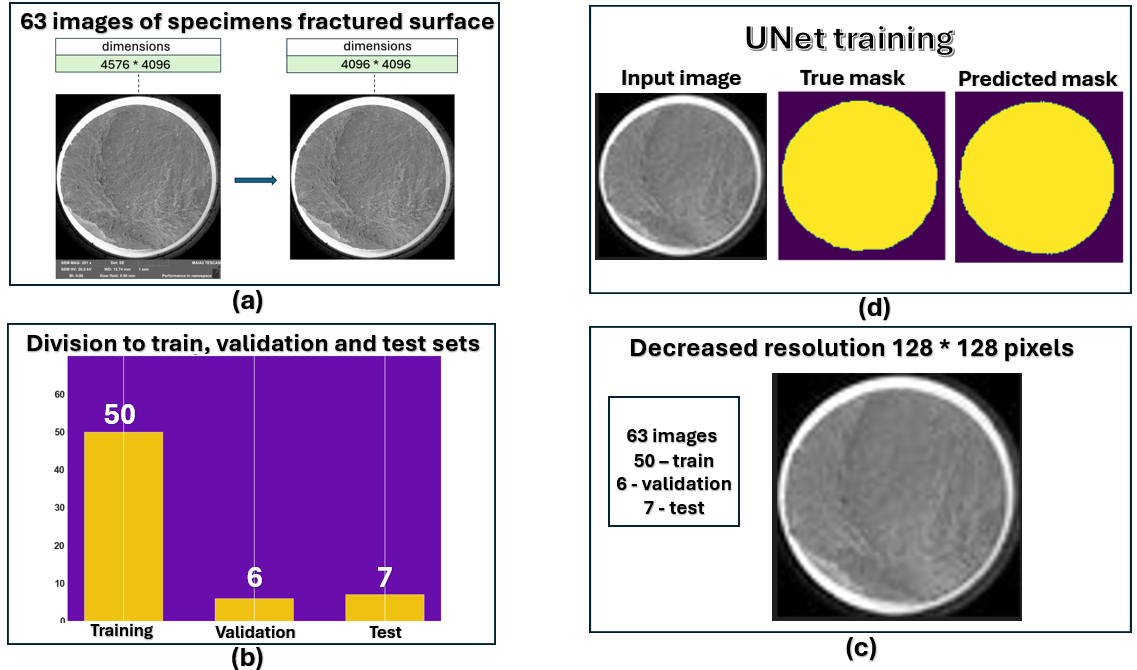
\includegraphics[width=1\linewidth, height=0.23\textheight]{figures/steps_dataset4.png}
  \caption{Dataset preparation: (a) Cropping images to remove metadata; (b) Train/test split; (c) Resizing to 128x128 for initial UNet; (d) Final images for model training.}
  \label{steps_was_done}
\end{figure}



\subsubsection{Manual Labeling for External Contour Detection}
After resizing the images, a manual labeling process was performed to detect the external contours of the specimens using a Python script that allowed for contour drawing and mask generation (Figure~\ref{lables}).
The labeled images were reviewed by fracture study experts to ensure accuracy and consistency, which was critical for training the model. This validation step ensured that the model learned relevant features for accurate external contour detection.

\subsubsection{Dataset Division and Resolution Adjustment}
The dataset was split into training, validation, and test sets, with images resized to 128x128 pixels to balance model complexity and performance. This resizing ensured computational efficiency without sacrificing accuracy (see Table~\ref{tab:dataset_division}).

\begin{table}[htbp]
\centering
\small
\caption{Division of the dataset into training, validation, and test sets}
\label{tab:dataset_division}
\begin{tabular}{@{}lcc@{}}
\toprule
\textbf{Dataset} & \textbf{Number of Images} & \textbf{Percentage (\%)} \\ \midrule
Training Set & 50 & 79.37 \\
Validation Set & 6 & 9.5 \\ \bottomrule
Test Set & 7 & 11.1 \\ \bottomrule
\textbf{Total} & \textbf{63} & \textbf{100} \\ \bottomrule
\end{tabular}
\end{table}

\subsubsection{Normalization of Pixel Values}
Pixel values were normalized to a scale of 0 to 1, ensuring uniformity and allowing the model to focus on image patterns rather than intensity variations. This step improved the model's generalization capabilities.

\subsubsection{Data Augmentation Strategy}
Data augmentation, including random flips, rotations, zooms, translations, and contrast adjustments, was employed to enhance model robustness and prevent overfitting. These augmentations helped the model generalize better across varying real-world conditions.

\begin{figure*}[!t]
  \centering
  \begin{minipage}{0.98\textwidth}
    \centering
    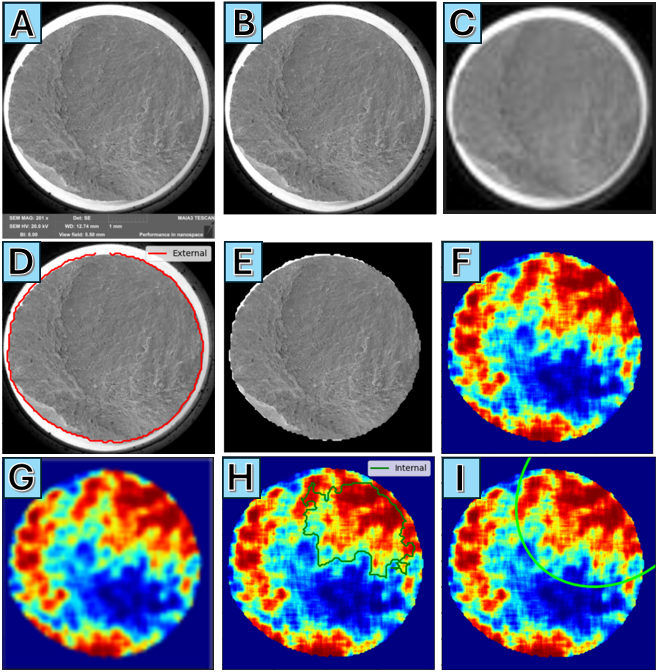
\includegraphics[width=0.672\textwidth]{figures/steps_dataset2.png}
    \caption{Sequential image processing steps: (A) SEM image, (B) Cropped image, (C) Resized image, (D) External contour detection, (E) Heatmap generation, (F) Final segmentation.}
    \label{steps}
  \end{minipage}
\end{figure*}

\subsubsection{Enhancing Image Details for Secondary Analysis}
Following the segmentation of external contours by the first UNet model, the resultant images, initially resized to 128x128 pixels for processing efficiency, are scaled back to their original resolution of 4096x4096 pixels. This resizing is pivotal for detailed secondary analysis, enabling the application of advanced image processing techniques essential for high-precision analysis. In this phase, edge definition is enhanced, and heatmaps are generated using Sobel operators and sliding window techniques, which are integral to capturing critical structural details.

To enhance the interpretability of images and emphasize important features, heat-maps are incorporated. Activation maps, such as Grad-CAM, prioritize the significance of image features or pixels identified by the model. Heat-maps visually represent these properties across the image surface, with varying colors indicating data intensity. This visualization is valuable for tasks such as pinpointing specific objects within an image and detecting anomalies—key aspects of fatigue failure analysis. Extracting these features allows neural network models to utilize validated prior knowledge, deepening the understanding of fatigue failure mechanisms \cite{selvaraju2017grad}.

Following the integration of heat maps to emphasize critical features, calculating the magnitude of gradients using the Sobel operator on an image is a technique used to enhance the image by detecting edges for easier analysis.
However, the edges detected by the Sobel operator tend to be thicker, which can affect the accuracy of feature extraction. This makes it challenging to rely solely on the Sobel operator without a deep understanding of the data being used.
Recent studies have demonstrated the necessity of gradient magnitude calculations, along with a technique to dilate the features, to improve detection accuracy on the edge of bridge cracks \cite{wang2019research}. 

The gradient magnitude indicates the intensity of the gradient at each pixel, calculated using the formula:
\begin{equation}
\label{eq:magnitude}
M=\sqrt{G_x^{^2}+G_y^{^2}}
\end{equation}
where $G_x$ and $G_y$ are the gradients in the $x$ and $y$ directions, respectively.

Gradient magnitude can be calculated using the Sobel operator, a discrete differentiation operator that computes an approximation of the gradient of the image intensity function. The result at each point in the image is either the corresponding gradient vector or the norm of this vector. The Sobel operator is based on convolving the image with a small, separable, and integer-valued filter in the horizontal and vertical directions, making it relatively inexpensive in terms of computations. Smoothing the gradient using a sliding window technique helps reduce noise and enhance the clarity of the gradient, facilitating easier detection and analysis of features in the image.

\begin{equation}
\label{eq:gradient}
G=\sqrt{\frac{1}{n^{^2}}\sum_{i=1}^{n}\sum_{j=1}^{n}I_{i,j}^{^2}}
\end{equation}
where $I_{i,j}$ is the intensity of the pixel in the $i$ row and $j$ column.
\begin{figure*}[!t] 
  \centering
  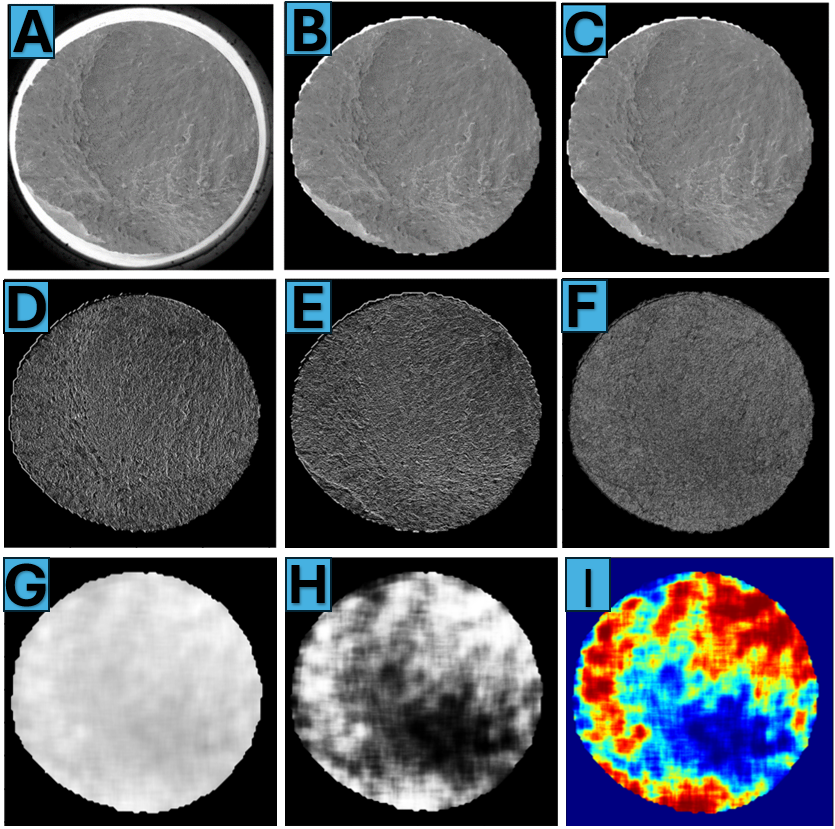
\includegraphics[width=0.672\linewidth]{figures/heatmap_generation.png}
  \caption{Transition from grayscale image to heatmap: (A) Original SEM image after crop metadata, (B) Grayscale image, (C) Gaussian blurred image, (D) Sobel operator applied in the x-axis, (E) Sobel operator applied in the y-axis, (F) Combined Sobel operator result, (G) Sliding window result, (H) Histogram equalization, (I) Final heatmap.}
  \label{fig:transition_heatmap}
\end{figure*}
The key steps in generating heatmaps (Figure~\ref{fig:transition_heatmap}) involve converting the SEM images to grayscale for efficient processing, applying Gaussian blurring to smooth intensity variations, and using the Sobel operator to detect both vertical and horizontal edges. The combined gradient magnitude at each pixel is calculated and normalized, followed by a sliding window technique to visualize edge intensity across the image. Finally, histogram equalization is applied to enhance contrast, and a color-coded heatmap is generated to highlight areas of interest.
This detailed process, from the initial image preprocessing and manual labeling to the generation of heatmaps, ensures that the data used for training the second UNet model is of high quality and relevance. These enhanced images facilitate accurate internal contour detection, which is critical for analyzing the intricate details of material fractures.
By thoroughly preparing the images through these steps, the study ensures that the neural network models are trained on robust, high-quality data, thereby improving the accuracy and reliability of the segmentation results. This methodical approach not only enhances the models performance but also contributes significantly to the understanding of material behavior under stress conditions, advancing the field of material science.

\subsubsection{Manual Labeling for Internal Contour Detection}
After heatmap generation, manual labeling was conducted for internal contours like cracks, ensuring precise segmentation. Expert review ensured consistency and accuracy, critical for training the second UNet model.

These steps—preprocessing, manual labeling, and data augmentation—ensured that the UNet models were trained on high-quality, relevant data, improving the accuracy and robustness of the segmentation results.

\begin{figure*}[!t]
  \centering
  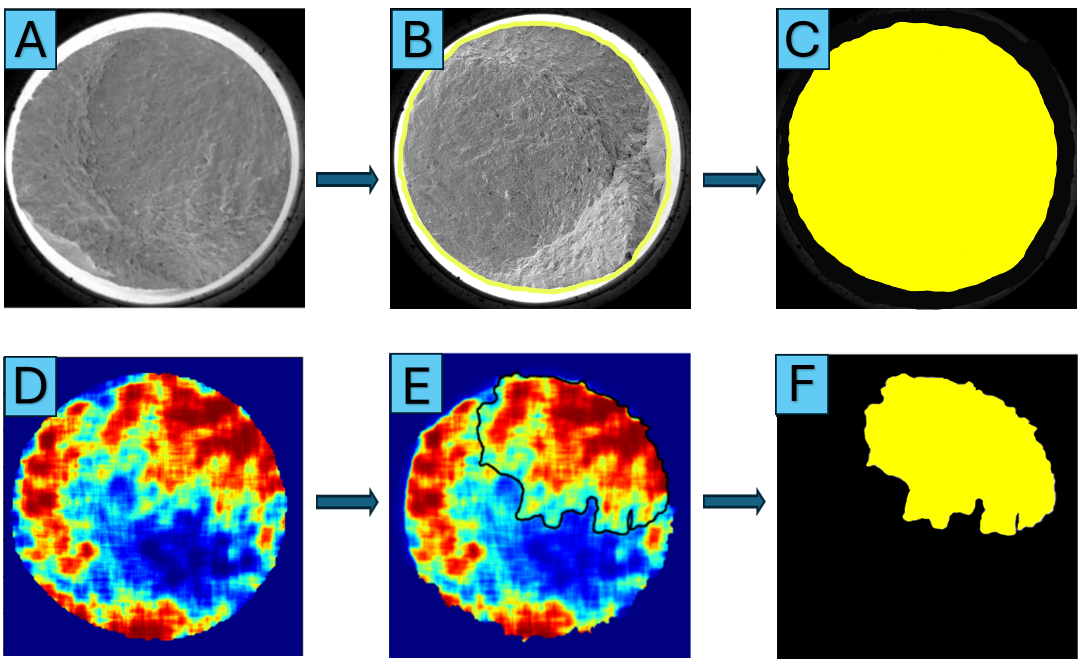
\includegraphics[width=0.8\textwidth]{figures/lables.png}
  \caption{Manual labeling process for external and internal contour detection: 'A' shows the cropped input image, 'B' is the manually identified external contour, 'C' is the generated mask for training the first UNet model. 'D' to 'F' depict crack detection and labeling for the second UNet model.}
  \label{lables}
\end{figure*}


\subsection{Customization of U-Net Architecture for Contour Detection}
\label{subsec:UNetArchitectureCustomization}
The U-Net architecture is adapted for the specific tasks of external and internal contour detection, enhancing its ability to process the complex textures and variations in SEM images.

\subsubsection{External Contour Detection}
For external contour detection, a U-Net model with a MobileNetV2 backbone, pre-trained on ImageNet, is employed for its efficient feature extraction capabilities.
\begin{itemize}
    \item \textbf{Model Configuration.} MobileNetV2, with depthwise separable convolutions, reduces computational load while capturing essential details. The expansive path of U-Net reconstructs the segmentation map, using skip connections to preserve detailed features.
    \item \textbf{Selection of MobileNetV2.} Its efficient architecture balances computational cost and accuracy, essential for high-resolution SEM images.
    \item \textbf{Pre-training on ImageNet.} Leveraging pre-trained weights on ImageNet enables the model to recognize complex patterns, accelerating training on SEM images.
    \item \textbf{Transfer Learning and Fine-Tuning.} Weights are fine-tuned for SEM images, using techniques like dropout and learning rate adjustments to mitigate overfitting.
    \item \textbf{Resolution Handling.} High-resolution SEM images are resized to 128x128 pixels to optimize computational resources while retaining essential details for contour detection.
\end{itemize}

\subsubsection{Internal Contour Detection Using Heatmaps}
For internal contour detection, the model processes heatmaps generated from external contour outputs, focusing on fracture detection. 
\begin{itemize}
    \item \textbf{Enhanced Feature Sensitivity.} The U-Net model's convolutional layers are fine-tuned for heatmaps, using a kernel size of 3x3 and stride of 1 for detailed feature extraction.
    \item \textbf{Weight Initialization and Adaptation.} Pre-trained weights from ImageNet are adapted for heatmap processing through additional training.
    \item \textbf{Precision in Feature Mapping.} Upsampling layers are calibrated to reconstruct high-resolution features, ensuring accurate internal contour segmentation.
    \item \textbf{Integration with Advanced Segmentation Techniques.} Techniques like batch normalization and dropout improve segmentation accuracy and generalization.
    \item \textbf{Training and Optimization.} The model uses the Adam optimizer for efficient convergence, with a batch size of 4 and early stopping to prevent overfitting.
    \item \textbf{Data Augmentation.} Augmentation techniques (flips, rotations, zooms, translations, and contrast adjustments) are applied to improve generalization.
    \item \textbf{Early Stopping and Epoch Management.} Early stopping halts training if validation loss doesn't improve for 60 epochs, ensuring computational efficiency.
\end{itemize}

\subsubsection{Application of Theoretical Concepts}
The U-Net architecture was customized using key theoretical concepts like convolutional layers, pooling, skip connections, and upsampling, specifically for SEM image analysis:
\begin{itemize}
    \item \textbf{Convolutional Layers.} 3x3 kernels with a stride of 1 were employed to capture intricate features in SEM images, preserving spatial resolution and learning fine details.
    \item \textbf{Pooling Layers:} Max pooling layers downsample images, reducing spatial dimensions while retaining important features, helping manage computational resources.
    \item \textbf{Skip Connections.} These retain high-resolution details from the downsampling process and reintroduce them during upsampling, essential for precise contour detection in SEM images.
    \item \textbf{Upsampling Layers.} Transposed convolutions increase spatial resolution, accurately reconstructing fine details in the segmentation output.
\end{itemize}

\subsubsection{Adaptation to SEM Image Analysis}
Several modifications were made to adapt the U-Net architecture to SEM images:
\begin{itemize}
    \item \textbf{Convolutional Layers.} Configured with 3x3 kernels and a stride of 1, fine-tuned through experimentation to balance feature capture and computational efficiency.
    \item \textbf{Pooling Layers.} Max pooling reduces image dimensions without losing essential information, necessary for handling high-resolution SEM images.
    \item \textbf{Skip Connections.} Ensures high-resolution information is preserved during upsampling, critical for accurate segmentation of SEM image features.
    \item \textbf{Upsampling Layers.} Precisely maps high-resolution features, ensuring sharp boundaries in internal contour detection.
\end{itemize}
By applying these concepts, U-Net is effectively customized to handle the complexity of SEM images, achieving high accuracy and robustness in microstructural feature segmentation.



\subsection{Flow Stress and Stress Intensity Factor Calculation}
\label{subsec:FlowStressSIFCalculation}
Upon detecting the external contour of the entire specimen and the internal contour of the crack propagation zone, the stress intensity factor (SIF) and flow stress are subsequently calculated.

The flow stress is evaluated according to the equation described in Section~\ref{Subsec: Flow stress calculation model}, leveraging the relationship between the areas enclosed by the external and internal contours, with the applied stress value being 634 MPa.

The calculation of the SIF is outlined in Section~\ref{Subsec: Stress intensity factor calculation model}. The parameters \(a\), \(b\), and \(D\) for the ellipse are derived through geometric analysis, with the SIF being calculated for both the crack front and the middle front, corresponding to \(x/h = 0\) and \(x/h = 1\), respectively.
The detailed steps for SIF calculation are as follows:

\begin{itemize}
    \item \textbf{Centroid Calculation:} Determine the centroids of both the external and internal contours, representing the center of gravity for each contour.
    \item \textbf{Vector Determination.} Calculate the vector extending from the centroid of the external contour to the centroid of the internal contour, representing the direction of crack propagation.
    \item \textbf{Elliptical Fitting.} Employ the \texttt{cv2.fitEllipse()} method to accurately fit an ellipse to the internal contour.
    \item \textbf{Maximal Length Calculation:} Measure the maximal length of the internal contour along the determined vector direction.
    \item \textbf{Axis Calculation.} Compute the new minor and major axes of the ellipse based on the maximal length measurement.
    \item \textbf{Extraction of SIF Parameters.} Derive the SIF parameters \(a'\), \(b'\), and \(D'\) from the newly calculated ellipse, as illustrated in Fig.~\ref{fig:ellipse_parameters}.
\end{itemize}

\begin{figure}[!t]
    \centering
    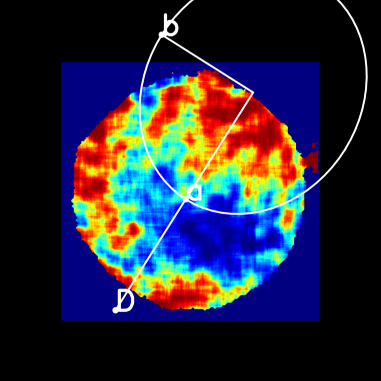
\includegraphics[width=0.4\textwidth]{figures/ellipse_parameters.png}
    \caption{Illustration of the elliptical parameters \(a'\), \(b'\), and \(D'\) derived from the calculated ellipse. The parameters are used to determine the stress intensity factor (SIF) for the crack front and the middle front.}
    \label{fig:ellipse_parameters}
\end{figure}


\section{Experimental Evaluation and Results} 
\label{sec:Experimental Evaluation and Results}

\subsection{Evaluation of Developed U-Net Model}
\label{subsec: Evaluation of Developed U-Net Mode}
A fundamental metric for evaluating classification models, and to a certain extent segmentation tasks, is the accuracy metric. For the U-Net model, accuracy is computed for each pixel within the image, followed by an aggregation to obtain the mean accuracy. This process involves classifying each pixel based on whether it falls within the predicted contour. Accuracy for an individual image is determined by the ratio of correctly classified pixels to the total number of pixels in that image. Consequently, the mean accuracy is derived from the average of these accuracy values across all images.
\begin{align*}
\text{Mean Accuracy} & = \frac{1}{N} \sum_{i=1}^{N} \frac{C_i}{T_i}, \\
N & = \text{Total number of images}, \\
C_i & = \text{Correct pixels in image } i, \\
T_i & = \text{Total pixels in image } i.
\end{align*}


Another common metrics, which specifically addresses the evaluation of model performance in segmentation tasks, are the Intersection over Union (IoU) and Dice Coefficient.
The IoU objective is to compare the intersection of the predicted segmentation with the ground truth relative to their combined area. The IoU is calculated as follows:
\begin{equation}
\text{IoU} = \frac{|X \cap Y|}{|X \cup Y|}
\end{equation}
where $X$ and $Y$ are the predicted segmentation and the ground truth, respectively.
The Dice coefficient, also known as the F1 score, evaluates the overlap between the twice the intersection of the predicted segmentation and the ground truth relative to the sum of their areas. The Dice coefficient is calculated as follows:
\begin{equation}
\text{Dice} = \frac{2|X \cap Y|}{|X| + |Y|}
\end{equation}
where $|X|$ and $|Y|$ are the areas of the predicted segmentation and the ground truth, respectively.
To mitigate the impact of class imbalance on the model's evaluation, the \( F_{\beta} \) score is used as the evaluation metric instead of the standard F1 score. The \( F_{\beta} \) score allows for a flexible balance between precision and recall by introducing the parameter \(\beta\), which adjusts the weight of recall relative to precision.
The \( F_{\beta} \) score is defined as:
\[
\text{F}_{\beta} = (1 + \beta^{^2}) \times \frac{\text{Precision} \times \text{Recall}}{(\beta^{^2} \times \text{Precision}) + \text{Recall}}
\]


where \(\beta\) determines the relative importance of recall in the calculation.


In this study, for the external contour detection model, \(\beta\) is set to 0.5 to emphasize precision over recall, whereas for the internal contour detection model, \(\beta\) is set to 1.5, emphasizing recall over precision.

In the training phase, the U-Net model was evaluated using loss and accuracy metrics for each epoch on both the training and validation datasets.
The model weights were selected from the epoch that yielded the lowest loss on the validation dataset.
An early stopping method based on the validation loss was employed to determine when to halt the training.
Specifically, training was stopped if there was no decrease in validation loss for a predetermined number of epochs.
The number of epochs set for early stopping was 60 for internal contour detection and 20 for external contour detection, and the total number of epochs was capped at 200.

The U-Net was trained on 50 images and evaluated on two separate sets: a validation set of 6 images for tuning the learning process, and a test set of 7 images to evaluate its generalization to new data. The training used the Adam optimizer and the Sparse Categorical Cross-Entropy (SCCE) loss function, suitable for pixel-wise classification tasks in image segmentation due to its computational efficiency and effectiveness in multi-class scenarios where classes are mutually exclusive. Unlike Categorical Cross-Entropy, SCCE is designed for cases where target values are integers, simplifying the model's output layer.

Training was structured into epochs, with the number of steps per epoch determined by dividing the total training images by a batch size of 4, resulting in 12 steps per epoch. Validation followed a similar setup, with one step per epoch based on the validation set size and the same batch size. Metrics for accuracy and loss were calculated after each epoch for both training and validation data, as shown in Figure \ref{fig:model_performance_graphs}.

The U-Net model uses pretrained ImageNet weights for its downsampling path, while its upsampling path is trained from scratch. This strategy leverages the rich feature representations learned from the large and diverse ImageNet dataset, facilitating better initial performance and faster convergence on the specific dataset in use.


\subsection{\textbf{U-Net Results}}
\label{Subsec: U-Net Results}

Evaluation metrics, including mean accuracy and the Intersection over Union (IoU), were used to evaluate the model's performance on the test dataset, with the results are presented in Table \ref{tab:unet_performance}. The accuracy metrics indicate an enhanced performance by the model in identifying internal contours on the validation dataset relative to the training dataset. This improvement is hypothesized to stem from the implementation of augmentation on the training dataset, an approach not adopted for the validation dataset. The use of an augmented training dataset likely makes it more challenging for the model to detect internal contours within the training dataset itself. This could contribute to the increased difficulty in detecting internal contours in the training dataset.

Furthermore, the lower IoU score compared to accuracy, as detailed in Table \ref{tab:unet_performance}, suggests that IoU is more focused on accurately outlining shapes rather than balancing shape types. Unlike accuracy, IoU more precisely captures the complexity of contour outlines and the aspect of class distribution.

The model demonstrates indeed convergence of the loss function, and minimal variance at the point marked by the green line, which represents the point with minimal validation loss (as presented in Figs.~\ref{fig:model_performance_graphs}c and~\ref{fig:model_performance_graphs}d).

\begin{table}[ht]
\centering
\begin{tabular}{lcccc}
\hline
Model & Best Epoch & Acc. (\%) & IoU (\%) & F1 (\%)\\ \hline
U-Net (Ext. Contours) & 18 & 99.0 & 97.8 & 99.3 \\
U-Net (Int. Contours) & 157 & 95.0 & 87.6 & 87.4 \\ \hline
\end{tabular}
\caption{Accuracy metrics for U-Net models on External and Internal Contour detection.}
\label{tab:unet_performance}
\end{table}

% print the model performance graphs


\begin{figure*}[!t]
    \centering
    % Adjust the width and height parameters as needed to fit the image without cropping
    \begin{adjustbox}{max width=0.8\linewidth, max height=0.8\textheight}
        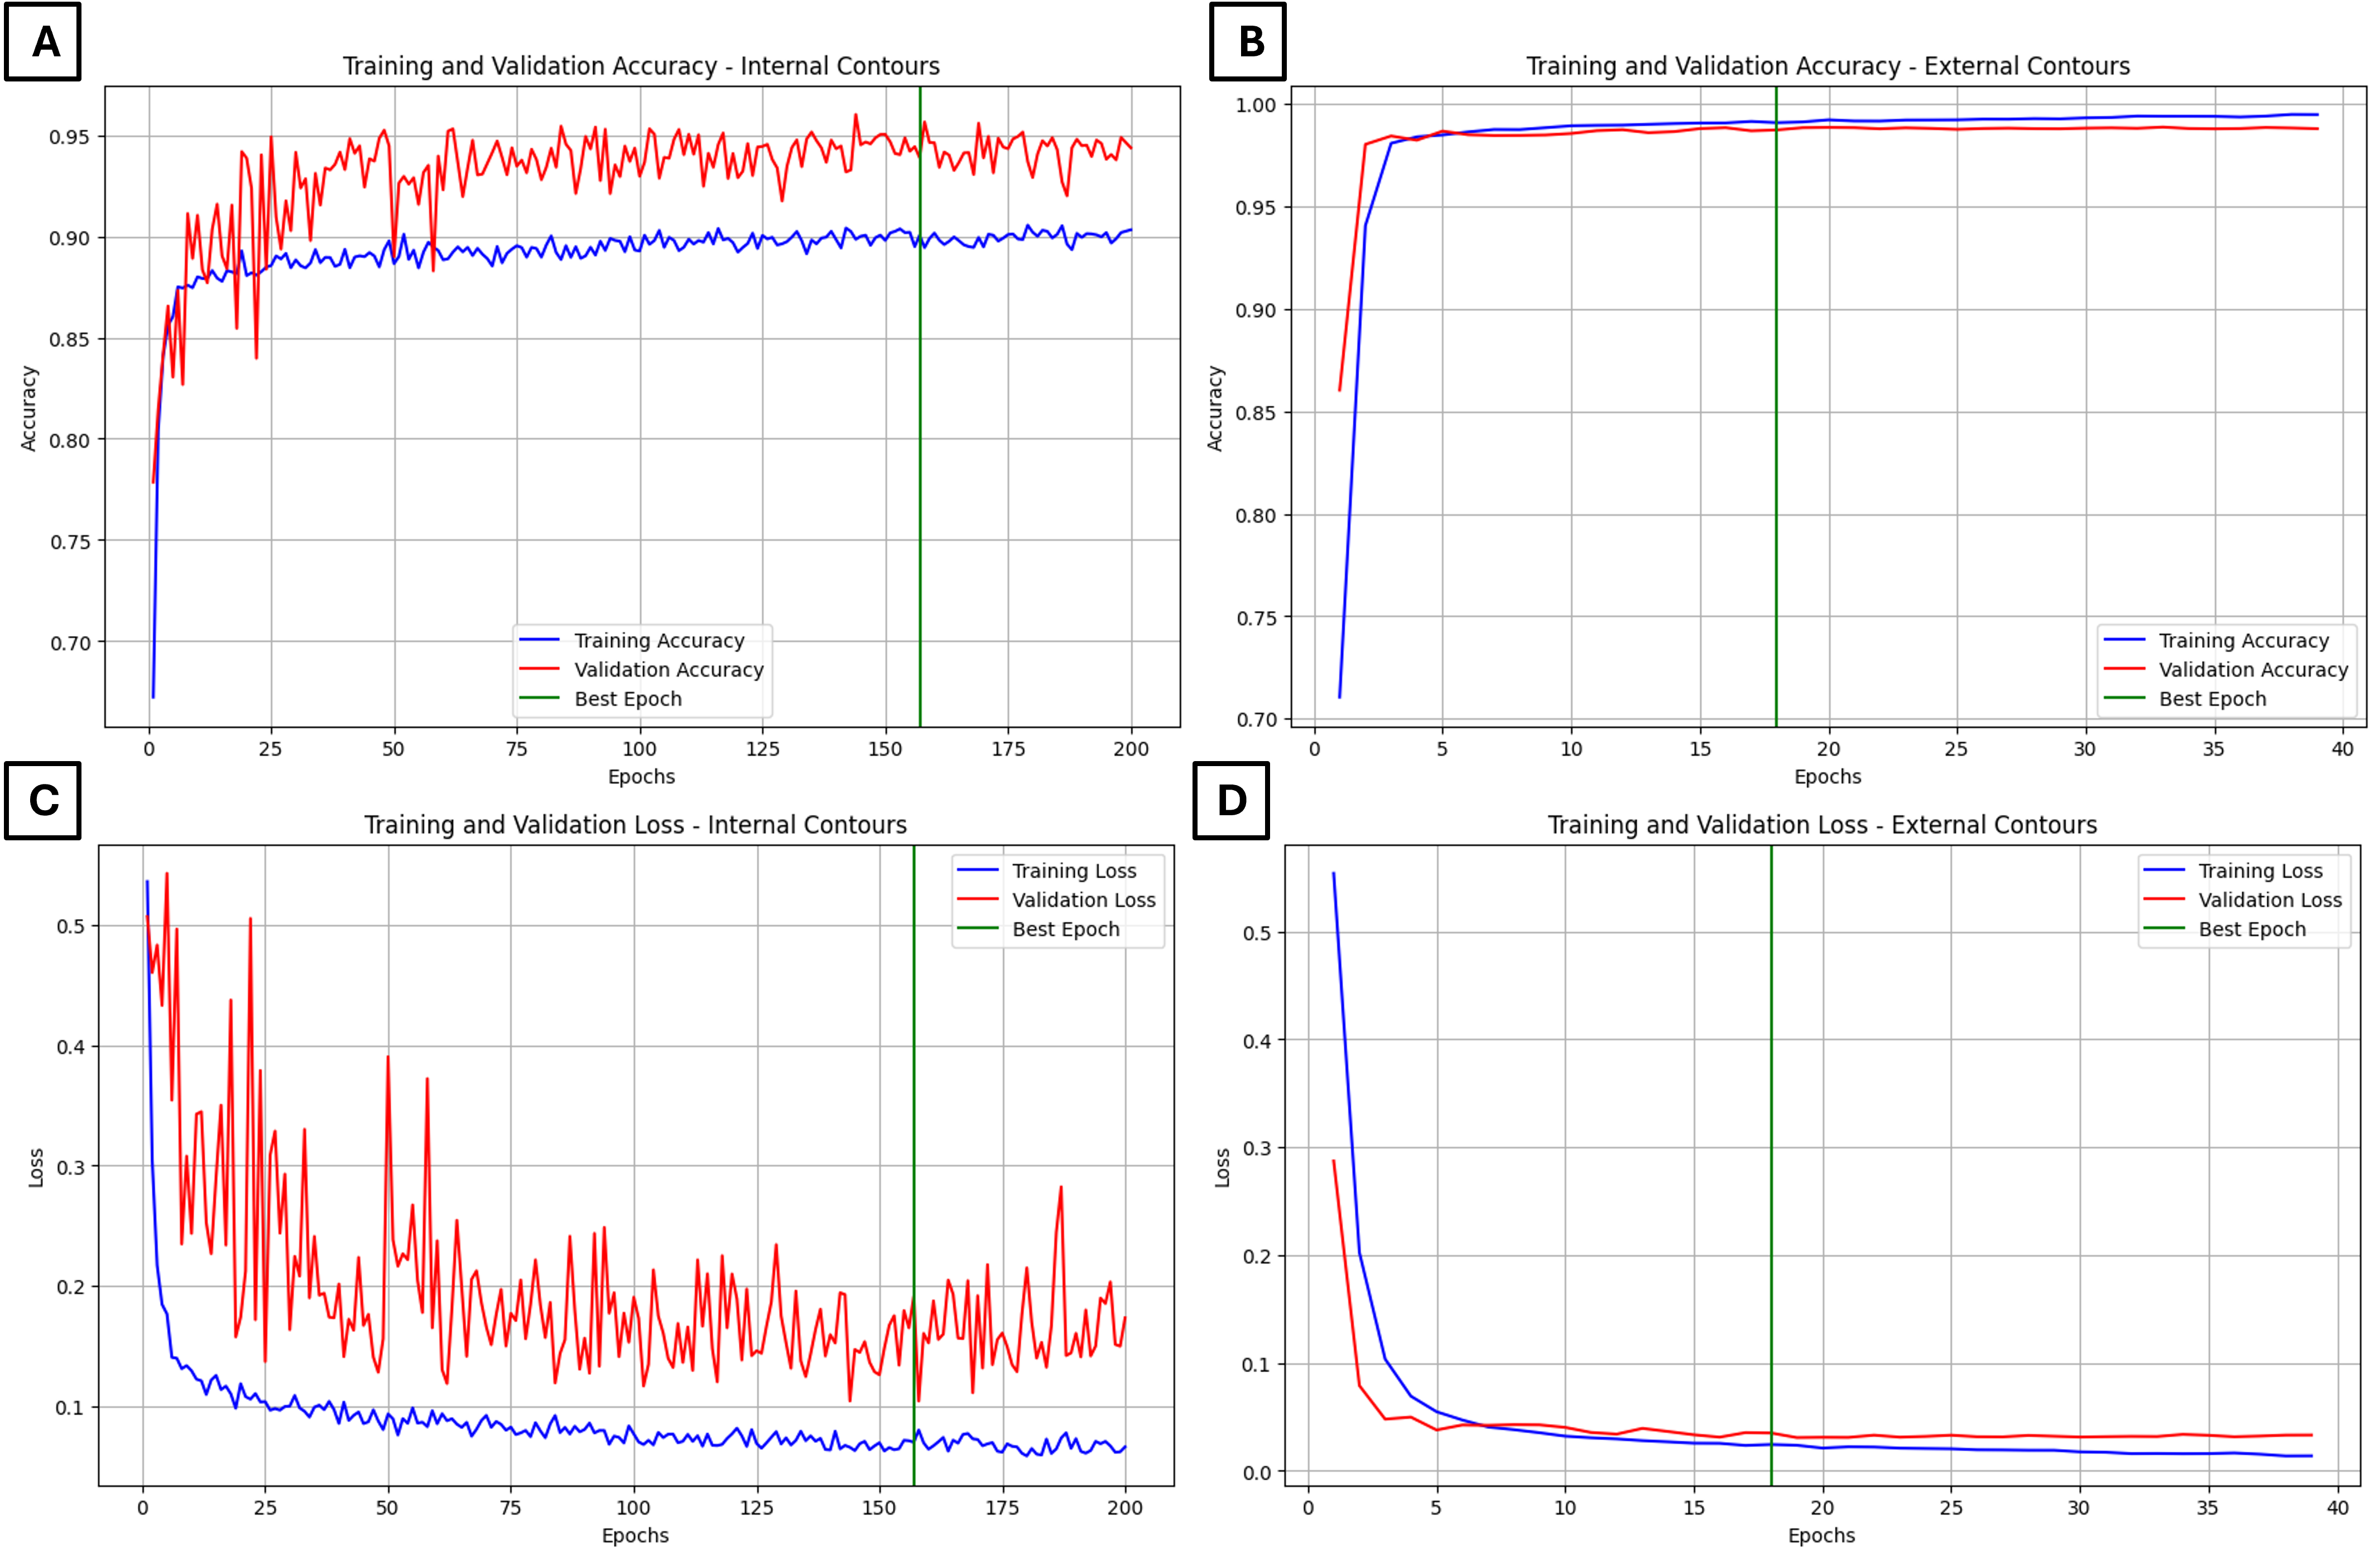
\includegraphics{figures/model_performance_graphs.png}
    \end{adjustbox}
    \caption{Performance graphs for the U-Net model. The graphs show the model's accuracy and loss metrics for both training and validation datasets across epochs. (a) Accuracy of the internal contour detection model. (b) Accuracy of the external contour detection model. (c) Loss of the internal contour detection model. (d) Loss of the external contour detection model.}
    \label{fig:model_performance_graphs}
\end{figure*}


\section{Validation cases}
\label{Sec: Validation cases}

\subsection{Fractographic Analysis - Manual Versus Image Processing}
\label{Subsec: Experimental Results}

This subsection details the fractographic analysis conducted utilizing the Sobel magnitude heatmap and the U-Net model, comparing these results with those obtained through validated processes.
Initially, it focuses on the evaluation of the Sobel magnitude heatmap, and subsequently, it presents the outcomes from the application of the U-Net model in locating the crack front and the whole fracture surface.

\subsubsection{Heatmap Evaluation}
\label{Subsubsec: Heatmap Evaluation}
The heatmap evaluation was conducted manually by experts in mechanical engineering.
By analyzing lower scale Scanning Electron Microscope (SEM) images, a sample from each distinct color area was selected for manual analysis from a set of specimens. Through this examination, the expert could identify the crack phase associated with each colored region of the heatmap. The color represents the scale of magnitudes over the surface, in which the scale of red colors represents the smoother region while the green to blue the rougher.  
The heatmap was segmented into five distinct areas, each representing a different phase of crack development: "dark red" for crack initiation, "red" and "light blue" for crack propagation, "blue" for final failure, and "broken" for areas unaffected by the crack, indicating the static phase of crack growth. From each of these areas, an image was selected, and its corresponding crack phase was manually identified by the expert. The outcomes of this manual analysis are depicted in Figure \ref{fig:heatmap_manual_analysis}.

Figure \ref{fig:heatmap_manual_analysis} displays the manual analysis results,
where the expert identified the crack initiation phase from the image in the red area,
the crack propagation phase from the image in the yellow area,
the final failure phase from the image in the green area, and the static phase of crack growth,
from the image in the blue area.


Consistency in the manual analysis process was maintained by establishing a set of fractographic guidelines. The crack initiation phase, represented by the dark red area, was commonly associated with lack of fusion and porosity, and characterized by fish-eye patterns in low magnification SEM images \cite{gunther2017fatigue}. At higher magnifications, this area is encircled by a fine granular structure. However, in the absence of porosity, identifying the crack initiation phase can be challenging. In such cases, it is characterized by smooth features and facets in low magnification SEM images, as shown in Fig.~\ref{fig:heatmap_manual_analysis}a.

The crack propagation phase, represented by the red and light blue areas, was identified by the presence of striations accompanying the crack tip, perpendicular to the crack propagation direction \cite{mcevily2010fatigue}. This phase is characterized by a rough surface in high magnification SEM images, as depicted in Fig.~\ref{fig:heatmap_manual_analysis}b and \ref{fig:heatmap_manual_analysis}c.


The final failure phase, represented by the blue area, is identified by the presence of a final fracture surface. This area exhibits an unstable fracture surface at high magnifications, indicating the fast fracture phase, as shown in Fig.~\ref{fig:heatmap_manual_analysis}d.

The static phase of crack growth, represented by the broken area, is characterized by either brittle or ductile fracture surfaces \cite{pineau2016failure}. This phase is distinguished by a rough surface and the presence of dimples, typical of ductile fracture features in high magnification SEM images, as shown in Fig.~\ref{fig:heatmap_manual_analysis}e.

\begin{figure*}[!t]
\centering
\includegraphics[width=0.7\textwidth]{figures/heatmap_manual_analysis.png}
\caption{Manual analysis of crack growth phases using a heatmap. The image shows a segmented heatmap with color-coded regions representing different stages of crack growth on the fracture surface. "Dark red" (a) denotes crack initiation, associated with lack of fusion and porosity, and characterized by fish-eye patterns. "Red" (b) and "light blue" (c) denote crack propagation, identified by striations perpendicular to the crack growth direction and a rough surface. "Blue" (d) denotes final failure, indicated by an unstable fracture surface, representing rapid crack growth. "Broken" (e) denotes the static crack growth area, displaying either brittle or ductile fracture surfaces, with rough surfaces and dimples typical of ductile fractures. Each region is supported by Scanning Electron Microscope (SEM) images, each with a field of view of 277 micrometers, visually representing the corresponding crack phase}
\label{fig:heatmap_manual_analysis}
\end{figure*}


\subsubsection{U-Net Model Application Evaluation}
\label{Subsubsec: U-Net Model Application Evaluation}
Two distinct U-Net models were employed to analyze the SEM images of the Ti-6Al-4V fatigue specimens.
The first model was trained to detect the external contour of the specimens, based on the external contour, while the second model was trained to identify the internal contour, learned from the heatmap.
The performance of these models was evaluated on SEM images not included in their training set. The outputs of the models were compared with manual segmentation of the contours, with the internal contour evaluated on the heatmap and the external contour evaluated on the original images, against the automated results produced by the U-Net models.

Figures \ref{fig:manual_vs_automated_detection}a and \ref{fig:manual_vs_automated_detection}b show the results of manual segmentation and automated detection using the U-Net model of the whole fracture surface, also known as the external contours, over the original image, respectively. Figures \ref{fig:manual_vs_automated_detection}d and \ref{fig:manual_vs_automated_detection}e present the manual and automated detection of the crack front, also known as the internal contour. Figures \ref{fig:manual_vs_automated_detection}c and \ref{fig:manual_vs_automated_detection}f demonstrate the high overlap between the predicted and ground truth contours for both external and internal contours, as indicated by the IoU parameter introduced in Section~\ref{Subsec:Hypothesis Validation}.


\begin{figure*}[!t]
\centering
\includegraphics[width=0.8\textwidth]{figures/manual_vs_automated_detection.png}
\caption{Comparison of manual and automated detection of the crack front and the whole fracture surface. (a) Manual detection of the fracture surface over the original image. (b) Automated detection using the U-Net model. (c) Comparison of manual and automated crack front detection, showing intersection (green), manual only (blue), and automated only (red) regions, with an IoU score of 0.97. (d) Manual detection of the crack front over the heatmap image. (e) Automated detection of the fracture surface using the U-Net model. (f) Comparison of manual and automated fracture surface detection, showing intersection (green), manual only (blue), and automated only (red) regions, with an IoU score of 0.93.}

\label{fig:manual_vs_automated_detection}
\end{figure*}


\subsection{Stress intensity factor and flow stress}
\label{Subsec: Stress intensity factor and flow stress}

The stress intensity factor (SIF) and flow stress values were analyzed by measuring these parameters at both the middle and edge of the crack front. The data were presented as averages along with their respective standard deviations to provide a comprehensive understanding of the material's behavior.

Specimens were categorized according to their processing conditions. Two primary categories were identified: those subjected to Hot Isostatic Pressing (HIP), a post-processing treatment, and those in the As-Built (AB) condition. HIP involves applying high temperature and pressure uniformly to eliminate internal voids and defects, thereby enhancing mechanical properties. According to a study by~\cite{leuders2013mechanical}, HIP-treated specimens exhibit improved structural integrity with significantly reduced residual stress defects. Conversely, AB specimens were analyzed in their original manufactured state without undergoing any post-processing treatments, allowing for a direct comparison of mechanical properties between treated and untreated samples.


Additionally, specimens were divided based on their tray numbers, labeled as P1, P2, and P3, as introduced in Section \ref{Sec:dataset}. This classification resulted in a total of five categorical combinations, except for the combination of P3 and AB, which was not present. This categorization aimed to evaluate the effects of different Additive Manufacturing (AM) printing parameters on the mechanical properties of the materials.

The graph was plotted with SIF and flow stress values against the cycles to failure. This visualization emphasizes that while the number of cycles to failure can vary significantly based on the manufacturing parameters and post-processing treatments, SIF and flow stress—being intrinsic properties of the material—are not expected to show substantial variation across different specimens. This distinction underscores the importance of processing techniques in influencing the durability and failure characteristics of the material, while the core mechanical properties, such as SIF and flow stress, remain relatively stable. This relationship is clearly illustrated in Figures \ref{fig:middle_crack_front}, \ref{fig:edge_crack_front} and \ref{fig:flow_stress}.

\begin{figure*}[!t]
    \centering
    \begin{minipage}{0.45\linewidth}
        \centering
        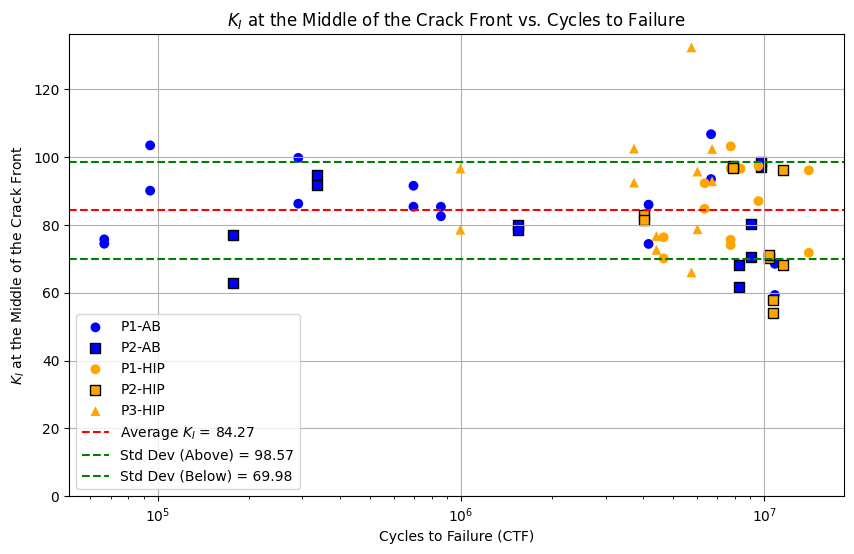
\includegraphics[width=\linewidth]{figures/KI Values at the Middle of the Crack Front vs. Cycles to Failure (CTF).png}
        \caption{$K_I$ at the Middle of the Crack Front vs. Cycles to Failure (CTF)}
        \label{fig:middle_crack_front}
    \end{minipage}
    \hfill
    \begin{minipage}{0.45\linewidth}
        \centering
        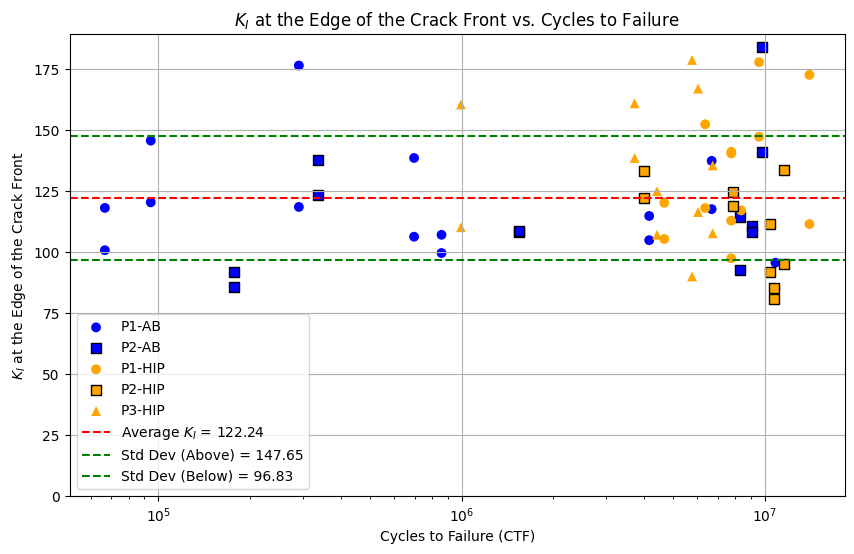
\includegraphics[width=\linewidth]{figures/KI Values at the Edge of the Crack Front vs. Cycles to Failure (CTF).png}
        \caption{$K_I$ at the Edge of the Crack Front vs. Cycles to Failure (CTF)}
        \label{fig:edge_crack_front}
    \end{minipage}
    
    \vspace{0.5cm} % Add some space between the rows

    \begin{minipage}{0.45\linewidth}
        \centering
        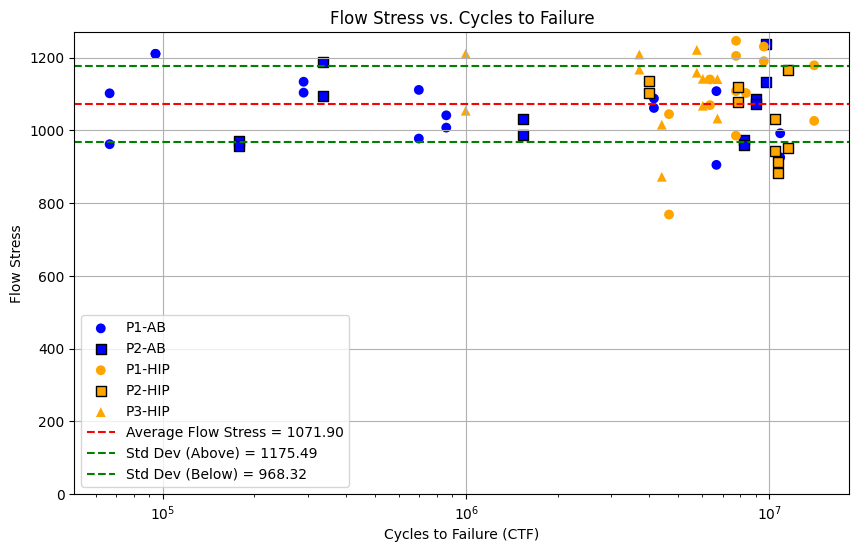
\includegraphics[width=\linewidth]{figures/Flow Stress vs Cycles to Failure.png}
        \caption{Flow Stress vs. Cycles to Failure (CTF)}
        \label{fig:flow_stress}
    \end{minipage}
    \label{fig:combined_graphs}
\end{figure*}

\section{Conclusions and Future Work}
\label{Sec: Conclusions and future work}

\subsection{Conclusions}
This study demonstrated the effective adaptation of the U-Net architecture for the segmentation of external and internal contours in scanning electron microscope (SEM) images, significantly enhancing both the accuracy and efficiency of material analysis. Through the integration of sophisticated neural network techniques, specifically tailored for the complexities of SEM data, the customized U-Net model has shown robust capabilities in detailed feature extraction and precise image segmentation.

A key innovation in this approach was the implementation of heatmaps for internal contour detection. These heatmaps have proven indispensable in identifying and localizing fracture zones within materials, providing a high level of detail that facilitates in-depth analysis of material behavior and failure mechanisms. Additionally, the development of automatic calculation methods utilizing these heatmaps has markedly improved the speed and reliability of analyses, reducing dependence on labor-intensive manual methods and enhancing the objectivity of the results (Section~\ref{Subsubsec: Heatmap Evaluation}).

As demonstrated in Section~\ref{Subsec: U-Net Results}, the U-Net model achieved high accuracy in detecting external and internal contours, with IOU values of 97.8\% and 87.6\%, respectively. Additionally, as mentioned in Section~\ref{Subsubsec: U-Net Model Application Evaluation}, the model successfully identified the internal and external contours of the fracture surfaces. This was confirmed through visual and quantitative comparisons with manual analyses, showcasing the model's effectiveness in detecting critical structural features.

However, the model performed poorly for specimens extracted from other imaging modalities, such as Stereomicroscope.

Further research is needed to enhance the model's adaptability to diverse imaging techniques and materials, ensuring its broad applicability in material science research and industrial quality control.


\subsection{Potential Uses and Developments}
\label{subsec:Potential Uses and Developments}
The methodologies developed in this study have broad applications in material science research and industrial quality control. The ability to accurately segment and analyze SEM images opens up new avenues for understanding material properties, failure mechanisms, and performance characteristics.
These methods can be applied to various industries, including but not limited to:

\begin{itemize}
    \item \textbf{Aerospace.} Titanium alloys are widely used in aerospace applications due to their high strength-to-weight ratio and corrosion resistance. The ability to accurately analyze microstructural features and defects in these materials is crucial for ensuring the safety and reliability of aerospace components. Additive Manufacturing (AM) still has a long way to go before it can be used in critical aerospace applications. The ability to detect and analyze defects in AM parts is essential for ensuring their structural integrity and performance. Additionally, AM tends to result in relatively high porosity, which can lead to reduced mechanical properties and fatigue life. ~\cite{montanari2023additive}
    \item \textbf{Automotive.} The automotive industry has recently turned to the use of lightweight materials, such as titanium, to downsize components, improve fuel efficiency, and reduce emissions. AM is employed to reduce overall life cycle costs.~\cite{nyamekye2023impact}
    \item \textbf{Biomedical.} Titanium alloys have wide applications in the biomedical field, such as dental implants and joint replacements. A weak point of Selective Laser Melting (SLM) is the presence of residual stresses, which have a significant impact on the mechanical properties of the material. These patterns of stresses are significant when producing trauma devices, where the material is subjected to high loads.~\cite{marin2023biomedical}
\end{itemize}

\subsection{Future Work}
\begin{itemize}
    \item \textbf{Algorithm Enhancement.} Future work will focus on enhancing noise reduction techniques and improving edge detection. Enhanced noise reduction will make the algorithms more robust against varying SEM image qualities, while advanced edge detection will improve the accuracy of contour segmentation, particularly in complex microstructures. These refinements are crucial for ensuring reliable segmentation across diverse SEM conditions, thereby enhancing the overall effectiveness of the model.
    \item \textbf{Material Diversity.} Expanding the model’s application to include a broader range of materials and conditions is essential for verifying its adaptability and effectiveness in diverse scientific fields. Future work will focus on making the model more robust to different resolutions and different materials, ensuring consistent performance across varied datasets. Additionally, the model’s adaptability to images from different imaging techniques, not just SEM, will be explored to enhance its versatility. Hypotheses for future exploration include testing the model on composites, metals, and polymers to assess its ability to detect material-specific features and provide detailed insights into structural integrity and failure mechanisms.
    \item \textbf{Real-time Analysis Capabilities.} Developing real-time processing features is a promising direction for dynamic testing environments where immediate results can significantly enhance workflow efficiency. Preliminary steps include optimizing the computational efficiency of the U-Net model and employing hardware accelerations like GPUs and TPUs. Real-time capabilities will be particularly impactful in applications such as in-situ monitoring and quality control, where rapid feedback is essential.}
    \item \textbf{User-Friendly Software Development.} Developing user-friendly software interfaces for non-experts to utilize the model in industrial and research settings is crucial. These interfaces will make advanced image analysis accessible to a broader audience, facilitating wider adoption and application of the methodologies developed in this study.
\end{itemize}

\bibliographystyle{unsrt}
\bibliography{bibs}

\begin{IEEEbiography}[{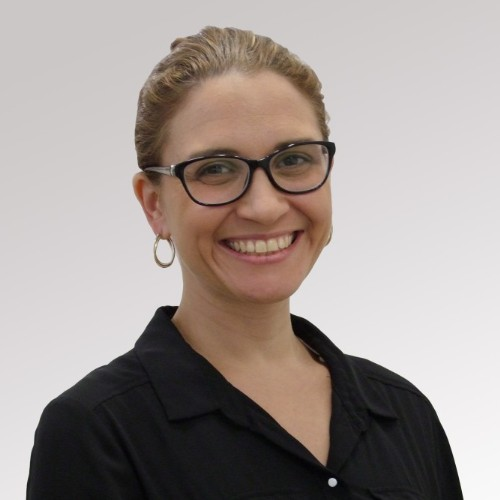
\includegraphics[width=1in,height=1.5in,clip,keepaspectratio]{Mor.jpeg}}]{Mor Mega} is a dedicated faculty member in the Department of Mechanical Engineering \& Mechatronics at the School of Engineering, Ariel University, Israel, holding the position of a Lecturer, which is equivalent to an Assistant Professor. She serves as the Head of the Fracture and Fatigue Research Laboratory (FFRL) and is responsible for leading the classical mechanics specialization course.
Dr. Mega's primary research area focuses on investigating the fracture and fatigue behavior of composite laminates and additive manufacturing components.
\end{IEEEbiography}

\begin{IEEEbiography}[{
\includegraphics[width=1in,height=1.5in,clip,keepaspectratio]{Or.png}}]{Or Haim Anidjar} is a Lecturer and a senior faculty member at the School of Computer Science at Ariel University, Israel. He forms a lab member at the (i) Kinematics and Computational Geometry (K\&CG) Lab; (ii) Ariel Cyber Innovation Center (ACIC); (iii) Data Science and Artificial Intelligence Research Center (DSAIRC); and (iv) Architectural AI Research Lab (AAIRL) at Ariel University, Israel. Or received his B.Sc. degree in Computer Science from Bar Illan University, Israel, and his M.Sc. and Ph.D degrees in Computer Science and Applied Mathematics from Ariel University, Israel, in 2015, 2019, and 2021 respectively. In 2022, Or was a Post-doctoral Fellow at the ACIC, Ariel University, Israel. By using Deep-Learning methods, his research lies at the intersection between Natural Language Processing (NLP) and Speech Recognition (SR), especially in multidisciplinary methods, such as Language Models, Speaker Change Detection and Diarization, Speaker Identification, and Anomaly Detection in acoustic and textual datasets. Formerly, Or was the Founder, CEO and Chief Data Scientist of Libonea.AI.
\end{IEEEbiography}

\begin{IEEEbiography}[{
\includegraphics[width=1in,height=1.5in,clip,keepaspectratio]{yonatan.jpg}}]{Yonatan Boritski} is an undergraduate B.Sc. student in Computer Science and Mathematics, with a major in Data Science and Machine Learning, at the School of Computer Science at Ariel University, Israel. Under the supervision of Dr. Mor Mega and Dr. Or Haim Anidjar, he conducted his research on applying Deep Learning methods to the field of material science as part of his final project workshop in computer science.
\end{IEEEbiography}

\begin{IEEEbiography}[{
\includegraphics[width=1in,height=1.25in,clip,keepaspectratio]{Avichay.jpg}}]{Avichay Mazin} is an undergraduate B.Sc. student in Computer Science and Mathematics, with a major in Data Science and Machine Learning, at the School of Computer Science at Ariel University, Israel. Under the supervision of Dr. Mor Mega and Dr. Or Haim Anidjar, he conducted his research on applying Deep Learning methods to the field of material science as part of his final project workshop in computer science.
\end{IEEEbiography}



\EOD

\end{document}
